\documentclass{vldb}
\usepackage{graphicx, subfigure, multirow, times}
\usepackage{balance, url, amsfonts, verbatim, mathtools}

  \renewcommand{\ttdefault}{cmtt}

\newcommand{\sectionskip}{-0em}
\newcommand{\subsectionskip}{-0em}
\usepackage{mdwlist}

\newenvironment{myitemize}
{
   \vspace{-1mm}
    \begin{list}{$\bullet$ }{}
        \setlength{\topsep}{0em}
        \setlength{\parskip}{0pt}
        \setlength{\partopsep}{0pt}
        \setlength{\parsep}{0pt}         
        \setlength{\itemsep}{.25em} 
}
{
    \end{list} 
    \vspace{-1em}
}

\title{Probabilistically Bounded Staleness\\ for Practical Partial Quorums}

\author{Peter Bailis, Shivaram Venkataraman, Michael J. Franklin, Joseph M. Hellerstein, Ion Stoica\\
\affaddr{University of California, Berkeley}\\
\affaddr{\{pbailis, shivaram, franklin, hellerstein, istoica\}@cs.berkeley.edu}}

\newdef{definition}{Definition}

\begin{document}

\interfootnotelinepenalty=10000
\hyphenation{prob-a-bil-is-tic-ally}

\maketitle

\begin{quote}
\textit{All good ideas arrive by chance.}---Max Ernst
\end{quote}


\begin{abstract}

Modern storage systems employing quorum replication are often
configured to use partial, non-strict quorums.  These systems wait
only for a subset of their replicas to respond to a request before
returning an answer, without guaranteeing that read and write replica
sets intersect.  While these partial quorum mechanisms provide only
basic eventual consistency guarantees, with no limit to the recency of
data returned, these configurations are frequently ``good enough'' for
practitioners given their latency benefits. In this work, we discuss
why partial quorums are often acceptable in practice by analyzing the
staleness of data they return.  Extending prior work on strongly
consistent probabilistic quorums and using models of Dynamo-style
anti-entropy processes, we introduce Probabilistically Bounded
Staleness (PBS) consistency, which provides expectations of bounds on
staleness across both versions and wall clock time.  We derive a
closed-form solution for versioned staleness and model real-time
staleness for representative Dynamo-style systems under internet-scale
production workloads.  We quantitatively demonstrate why, in practice,
systems employing partial quorums often serve consistent data.

\end{abstract}


\vspace{\sectionskip}\section{Introduction}

Modern distributed storage systems need to be scalable, highly
available, and fast.  These systems typically replicate data across
different machines and often across datacenters for two reasons:
first, to provide high availability when components fail and, second,
to provide improved performance by serving requests from multiple
replicas.  In order to provide predictably low read and write latency,
systems often eschew protocols guaranteeing consistency of
reads\footnote{Note that this distributed replica consistency is
  differs from transactional consistency provided by ACID
  semantics~\cite{nosql, urbanmyths}\vspace{-2em}.} and instead opt
for eventually consistent protocols~\cite{cassandradefault,
  abadilatconsist, dynamo, feinbergpc, reddit, riaktalkone, outbrain}.
However, weak eventually consistent systems make no guarantees on the
staleness (recency in terms of versions written) of data items
returned except that the system will ``eventually'' return the most
recent version in the absence of new writes~\cite{vogels-defs}.

Distributed quorums can be used to ensure strong consistency across
multiple replicas of a data item by overlapping read and write replica
sets. However, waiting for responses from the potentially large
resulting quorum sizes increases operation latency, an important
consideration for service operators~\cite{perf-impact}. For example,
at Amazon, 100 ms of additional latency resulted in a 1\% drop in
sales~\cite{amazon-latency}, while 500 ms of additional latency in
Google's search resulted in a corresponding 20\% decrease in
traffic~\cite{google-talk}.  At scale, increased latencies correspond to
large amounts of lost revenue.

Employing \textit{partial} (or non-strict) quorums lowers latency in
quorum replication.  With partial quorums, sets of replicas written to
and read from are not guaranteed to overlap: given $N$ replicas and
read and write quorum sizes $R$ and $W,$ partial quorums imply
$R$$+$$W$$\leq$$N$.  Modern quorum-based data systems such as
Dynamo~\cite{dynamo} and its open source descendants Apache
Cassandra~\cite{cassandra-sigmod}, Basho Riak~\cite{riak}, and Project
Voldemort~\cite{voldemortpub} offer a choice between these two modes
of replication: strict quorums, providing strong
consistency, and partial quorums, providing eventual consistency.

In light of this fundamental latency-consistency trade-off, operators
frequently employ partial quorums~\cite{cassandra-docs,
  cassandradefault,feinbergpc,reddit, outbrain, maxperfblog} despite
the weak guarantees provided by eventual consistency---a controversial
decision~\cite{hamilton-cap, cops, walter, urbanmyths}.  Partial quorums are often acceptable to operators given their latency benefits, which are especially important as latencies grow (e.g., wide-area network deployments)~\cite{abadilatconsist, feinbergpc,
  hamilton-cap, helland}. Moreover, many programs can be carefully
designed to handle staleness through design patterns such as
compensation (e.g., memories, guesses, and apologies)~\cite{helland}
and associative and commutative operations (e.g., timelines, logs, and
notifications)~\cite{calm}.  In general, however, \textit{unbounded}
staleness poses significant challenges and is undesirable in practice.
The proliferation of partial quorum configurations suggests that many
applications can tolerate occasional cases of staleness and that stale
data tends to be ``fresh enough'' in most cases.

While common practice suggests that weak eventual consistency is a
viable solution for many operators, to date, this observation has been
mostly anecdotal. In this work, we quantify the degree to which
eventual consistency is both eventual and consistent and explain
why. Under worst-case conditions, eventual consistency results in an
unbounded degree of data staleness, but, as we will show, the average
case is often different.  Eventually consistent data stores cannot
promise immediate and perfect consistency but, for varying degrees of
certainty, can offer staleness bounds with respect to time (``how
eventual'') and version history (``how consistent'').

There is little prior work describing how to make these consistency
and staleness predictions under practical conditions.  The current
state of the art requires that users make rough guesses or perform
online profiling to determine the consistency provided by their data
stores. Moreover, users have even less guidance regarding how to chose
an appropriate replication configuration or how to predict the
behavior of partial quorums in production
environments.

To do better, we need to know when and why eventually consistent
systems return stale data and how to quantify the staleness of the
data they return.  In this work, we answer these questions in the
context of quorum replicated data stores by expanding theoretical
research on \textit{probabilistic quorums}~\cite{prob-quorum,
  quorum-overview} to account for multi-version staleness,
anti-entropy (asynchronous write propagation)~\cite{antientropy}, and
message dissemination protocols as used in today's systems.  More
precisely, we present algorithms and models for predicting the
staleness of partial quorums, called Probabilistically Bounded
Staleness (PBS) for partial quorums. There are two common axes for
measuring staleness in the literature: versions~\cite{podc-hpl, aqua,
  frac} and wall clock time~\cite{podc-hpl, vahdat-article,
  vahdat-bounded}.  PBS can be used to analyze both measures,
describing the probability of reading a version $t$ seconds after it
is written ($t$-visibility, or ``how eventual is eventual
consistency?''), of reading one of the last $k$ versions of a data
item ($k$-staleness, or ``how consistent is eventual consistency?''),
and of experiencing a combination of the two ($\langle k, t
\rangle$-staleness). PBS does not propose new mechanisms to enforce
deterministic staleness bounds~\cite{ aqua, trapp,vahdat-article,
  vahdat-bounded, frac}; instead, our goal is to provide a lens for
analyzing, improving, and predicting the behavior of
\textit{existing}, widely-deployed systems.

We provide closed-form solutions for PBS $k$-staleness and use Monte
Carlo methods to explore the trade-off between latency and
$t$-visibility.  We present a detailed study of Dynamo-style PBS
$t$-visibility using production latency distributions. We show how
relatively long-tailed one-way write latency distributions affect the
time required for a high probability of consistent reads.  For
example, in one production environment, switching from spinning disks
to solid-state drives dramatically improved staleness (e.g., $1.85$ms
versus $45.5$ms wait time for a $99.9$\% probability of consistent
reads) due to decreased write latency mean and variance.  We also make
quantitative observations of the latency-consistency trade-offs
offered by partial quorums.  For example, in another production
environment, we observe an $81.1\%$ latency improvement at the
$99.9$th percentile ($230$ to $43.3$ms) for a $202$ms window of
inconsistency ($99.9\%$ probability consistent reads).  While the
benefit of these trade-offs is application-specific, our analysis
demonstrates many of the performance benefits that lead many operators
to choose weak consistency.

We make the following contributions in this paper:

\begin{myitemize}

\item We develop the theory of Probabilistically Bounded Staleness
  (PBS) for partial quorums. PBS describes the probability of
  staleness across both versions ($k$-staleness) and time
  ($t$-visibility) as well as the probability of monotonic reads
  consistency.

\item We provide a closed-form analysis of $k$-staleness demonstrating
  how the probability of receiving data $k$ versions stale is
  exponentially reduced by $k$.  As a corollary, $k$-staleness tolerance also
  exponentially lowers quorum system \textit{load}.

\item We provide a model for $t$-visibility in Dynamo-style partial
  quorum systems, \textit{WARS}, showing how staleness is dependent on
  message reordering due to latency.  We evaluate the $t$-visibility
  of Dynamo-style systems using a combination of synthetic and
  production latency models.

\end{myitemize}

\vspace{\sectionskip}\section{Background}
\label{sec:background}

In this section, we provide background regarding quorum systems both
in theoretical academic literature and in practice.  We begin by
introducing prior work on traditional and probabilistic quorum
systems.  We next discuss Dynamo-style quorums, currently the most
widely deployed protocol for storage systems employing quorum
replication.  Finally, we survey reports of practitioner usage of
partial quorums for three Dynamo-style data systems.

\vspace{\subsectionskip}\subsection{Quorum Foundations: Theory}

Quorum systems have long been proposed as a replication strategy for
distributed data~\cite{quorums-start}.  Under quorum replication, a
data storage system writes a data item by sending it to a set of
replicas, called a write quorum.  To serve reads, the data system
fetches the data from a possibly different set of replicas, called a
read quorum.  For reads, the storage system compares the set of values
returned by the replicas, and, given a total ordering over versions of
the data item\footnote{This total ordering can be achieved using
  globally synchronized clocks~\cite{synch-clocks} or using a causal
  ordering provided by mechanisms such as vector
  clocks~\cite{vectorclock} with commutative merge
  functions~\cite{cops}}, can return the most recent value (or all
values received, if desired).  For each operation, read and write
quorums are chosen from a set of sets of replicas, known as a
\textit{quorum system}, with one system per data item.  There are many
ways to configure quorum systems, but one simple solution is to use
read and write quorums of fixed sizes, which we will denote $R$ and
$W$, respectively, for a set of nodes of size $N$.  To reiterate, a
quorum replicated data system uses one quorum system per data item.
Across data items, the quorum systems need not be identical

Informally, a strict quorum system is a quorum system with the
property that any two quorums (sets) in the quorum system overlap
(have non-empty intersection). This ensures consistency.  The minimum
sized quorum defines the system's fault tolerance, or availability.  A
simple example of a strict quorum system is the majority quorum
system, in which each quorum is of size $\lceil \frac{N}{2}\rceil$.
However, the theory literature contains many alternative quorum system
designs providing varying asymptotic properties of capacity,
scalability, and fault tolerance, from tree-quorums~\cite{treequorum}
to grid-quorums~\cite{quorumsystems} and highly-available
hybrids~\cite{92-quorums}.  Jim\'{e}nez-Peris et. al provide an
overview of traditional, strict quorum
systems~\cite{quorums-alternative}.

Partial quorum systems are natural extensions of strict quorum
systems: at least two quorums in a partial quorum system do not
overlap.  There are two relevant variants of partial quorum systems in
the literature: probabilistic quorum systems and k-quorums.

\textit{Probabilistic quorum systems} provide probabilistic guarantees
of quorum intersection.  By scaling the number of replicas, we can
achieve an arbitrarily high probability of
consistency~\cite{prob-quorum}.  Intuitively, this is a consequence of
the Birthday Paradox: as the number of replicas increases, the
probability of non-intersection between any two quorums decreases.
Probabilistic quorums have not been used to study bounded staleness,
particularly in the presence of anti-entropy, or asynchronous write
propagation~\cite{antientropy}.  Merideth and Reiter provide an
overview of these systems~\cite{quorum-overview}.

As an example of a probabilistic quorum system, given $N$ replicas and
randomly chosen read and write quorums of sizes $R$ and $W$, we can
calculate the probability that the read quorum does not contain the
last written version.  This probability of inconsistency is the number
of quorums of size $R$ composed of nodes that were not written to in
the write quorum divided by the number of possible quorums of size
$R$:
\begin{equation}
\label{eq:prob-strict}
p_{s}=\frac{{N-W \choose R}}{{N \choose R}}
\end{equation}
The probability of inconsistency is high except for large $N$.  With
$N=100$, $R=W=30$, $p_{s} = 1.88 \times
10^{-6}$~\cite{non-strict}.  However, with $N=3$, $R=W=1$, $p_{s}
= .\overline{6}$.  The asymptotics of these systems are
excellent---but only asymptotically.

\textit{$k$-quorum systems} provide \textit{deterministic} guarantees
that a partial quorum system will return values that are within $k$
versions of the most recent write~\cite{non-strict}.  In the single
writer scenario, a round-robin write scheduling scheme where each
write is sent to $\lceil\frac{N}{k}\rceil$ replicas ensures that any
replica is no more than $k$ versions out-of-date.  However, with
multiple writers, the global ordering properties that the
single-writer was able to control are lost, and the best known
algorithm for the pathological case results in a lower bound of
$(2N-1)(k-1)+N$ versions staleness~\cite{multi-k-quorum}.

This prior work makes two important assumptions. First, it typically
models quorum sizes as fixed, where the set of nodes with a version
does not grow over time.  Prior work examined ``dynamic systems'',
considering quorum membership churn~\cite{prob-quorum-dynamic},
network-aware quorum placement~\cite{delay-quorum, quorum-placement},
and network partitions~\cite{partitionedquorum} but not write
propagation. Second, it frequently assumes Byzantine failure.  We
revisit these assumptions in the next section.

\vspace{\subsectionskip}\subsection{Quorum Foundations: Practice}
\label{sec:practice}

In practice, many distributed data management systems use quorums as a
replication mechanism. Amazon's Dynamo~\cite{dynamo} is the progenitor
of a class of eventually-consistent key-value stores that includes
Apache Cassandra\footnote{Apache Cassandra.
  \url{cassandra.apache.org}}, Basho Riak\footnote{Basho Riak.
  \url{www.basho.org}}, and LinkedIn's Project
Voldemort\footnote{Project Voldemort.
  \url{www.project-voldemort.com}}.  All use the same variant of
quorum-style replication, and we are not aware of any significantly
different, widely adopted data systems using quorum replication.
However, with some work, we believe that other styles of replication
can adopt our methodology.  We describe key-value stores here, but any
replicated data store can use quorums, including full RDBMS systems.

Dynamo-style quorum systems employ one quorum system per key,
typically maintaining the mapping of keys to quorum systems using a
consistent-hashing scheme or a centralized membership protocol. Each
node stores multiple keys.  As shown in
Figure~\ref{fig:dynamo-quorum}, client read and write requests are
sent to a node in the system cluster, which forwards the request to
\textit{all} nodes assigned to that key as replicas.  This
coordinating node considers an operation complete when it has received
responses from a pre-determined number of replicas (typically set
per-operation).  Accordingly, without message loss, all replicas
eventually receive all writes.  This means that the write and read
quorums chosen for a request depend on which nodes respond to the
request first.  In Dynamo terminology, the quorum size, or replication
factor, is defined as $N$, the number of replica responses required
for a successful read is defined as $R$, and the number of replica
acknowledgments required for a successful write is defined as
$W$. Dynamo-style systems are guaranteed to be consistent when $R+W >
N$.  Setting $W>\lceil N/2 \rceil$ ensures that a majority of replicas
will will receive a write in the presence of multiple concurrent write
requests.

\begin{figure}
\centering
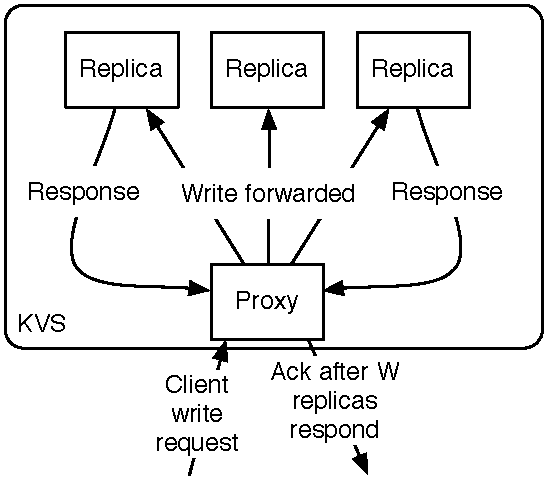
\includegraphics[width=.85\columnwidth]{figs/dynamo-quorum.pdf}
\vspace{-8pt}
\caption{Diagram of control flow for client write to Dynamo-style
  quorum ($N=3$, $W=2$).  The client write is handled by a
  coordinator node and sent to all $N$ replicas. The write call returns
  after the coordinator receives $W$ acknowledgments.}
\vspace{-12pt}
\label{fig:dynamo-quorum}
\end{figure}

There are significant differences between quorum theory and data
systems used in practice.  First, replication factors for distributed
data systems are relatively low.  Typical replication factors are
between one and three~\cite{cassandradefault, feinbergpc, codapc}.
Second, (in the absence of failure), in Dynamo-style partial quorums,
the write quorum size increases even after the operation returns,
growing via anti-entropy~\cite{antientropy}.  Moreover, requests are
sent to all replicas, however only the first $R$ responses are
considered.  As a matter of nomenclature (and to disambiguate against
``dynamic'' quorum membership protocols), we will refer to these
systems as \textit{expanding partial quorum systems}. (We discuss
additional anti-entropy in Section~\ref{sec:anti-entropy}.) Third, as
in much of the applied literature, practitioners focus largely on
fail-stop instead of Byzantine failure
modes~\cite{birman-byzantine}.  Following standard practice, we do not
consider Byzantine failure.

%\vspace{2em}

\vspace{\subsectionskip}\subsection{Typical Quorum Configurations}

For improved latency, operators often set $R+W \leq N$.  Here, we
survey quorum configurations according to practitioner accounts.  Many
operators appear to use partial quorum configurations, frequently
citing performance benefits and high availability. Interestingly, many
these accounts did not discuss the possibility or occurrence of
staleness resulting from partial quorum configurations.

Cassandra defaults to $N$$=$$3$,
$R$$=$$W$$=$$1$~\cite{cassandradefault}. The Apache Cassandra 1.0
documentation claims that ``a majority of users do writes at
consistency level [$W$$=$$1$]'', while the Cassandra Query Language
defaults to $R$$=$$W$$=$$1$ as well~\cite{cassandra-docs}.  Production
Cassandra users report using $R$$=$$W$$=$$1$ in the ``general case''
because it provides ``maximum performance''~\cite{maxperfblog}, which
appears to be a commonly held belief~\cite{reddit, outbrain}.
Cassandra has a ``minor'' patch~\cite{cassandra-session} for session
guarantees~\cite{sessionguarantees} that is not currently
used~\cite{cassandra-session-revert}; according to our
discussions with developers, this is due to lack of interest.

Riak defaults to $N$$=$$3$, $R$$=$$W$$=$$2$~\cite{riakdefault-n,
  riakdefault-rw}. Users suggest using $R$$=$$W$$=$$1$, $N$$=$$2$ for
``low value'' data (and strict quorum variants for ``web,''
``mission critical,'' and ``financial'' data)~\cite{riaktalkone,
  riaktalktwo}.

 Finally, Voldemort does not provide sample configurations, but
 Voldemort's authors (and operators) at LinkedIn~\cite{feinbergpc}
 often choose $N$$=$$c$, $R$$=$$W$$=$$ \lceil c/2 \rceil$ for odd $c$.
 For applications requiring ``very low latency and high
 availability,'' LinkedIn deploys Voldemort with $N$$=$$3$,
 $R$$=$$W$$=$$1$.  For other applications, LinkedIn deployments
 Voldemort with $N$$=$$2$, $R$$=$$W$$=$$1$, providing ``some
 consistency,'' particularly when $N$$=$$3$ replication is not
 required.  Additionally, Voldemort supports a concept of preferred
 reads and writes, meaning it will block until either the preferred
 number of replicas respond or a timeout occurs, at which point the
 request succeeds. Preferred reads is often set to two or disabled.  Voldemort
 also differs from Dynamo in that it sends read requests to $R$ of $N$
 replicas (not $N$ of $N$)~\cite{voldemortpub}; this decreases load
 per replica and network traffic at the expense of read latency and
 potential availability.  Provided the per-request staleness
 probabilities are independent, this does not affect staleness: even
 when sending reads to $N$ replicas, coordinators only wait for $R$
 responses.


\vspace{\sectionskip}\section{Probabilistically Bounded\\Staleness}
\label{sec:pbs}

In this section, we introduce Probabilistically Bounded Staleness,
which describes the consistency provided by existing eventually
consistent data stores.  We introduce the notions of PBS
$k$-staleness, which probabilistically bounds the staleness of versions
returned by read quorums, PBS $t$-visibility, which probabilistically
bounds the time before a committed version appears to readers, and PBS
$\langle k, t \rangle$-staleness, a combination of the two prior
models.

We first introduce $k$-staleness because it is self-contained, with a
simple closed-form solution.  In comparison, $t$-visibility is more
difficult, involving several additional variables.  Accordingly, this
section proceeds in order of increasing difficulty, and the remainder
of the paper largely addresses the complexities of $t$-visibility.

Practical concerns guide the following theoretical contributions.  We
begin by considering a model without quorum expansion or other
anti-entropy.  For the purposes of a running example, as in
Equation~\ref{eq:prob-strict}, we assume that $W$ ($R$) of $N$
replicas are randomly selected for each write (read) operation.
Similarly, we consider fixed $W$, $R$ and $N$ across multiple
operations. Next, we expand our model to consider write propagation
and time-varying $W$ sizes in expanding partial quorums.  In this
section, we discuss anti-entropy in general, however we model
Dynamo-style quorums in Section \ref{sec:dynamo}. We discuss further
refinements to these assumptions in Section \ref{sec:discussion}.

\vspace{\subsectionskip}\subsection{PBS $k$-staleness}
\label{sec:kstale}

Probabilistic quorums allow us to determine the probability of
returning the most recent value written to the database, but do not
describe what happens when the most recent value is not returned.
Here, we determine the probability of returning a value within a
bounded number of versions.  In the following formulation, we consider
traditional, non-expanding write quorums (no anti-entropy):
\begin{definition}
A quorum system obeys \textit{PBS $k$-staleness consistency} if, with
probability $1-p_{sk}$, at least one value in any read quorum will
have been committed within $k$ versions of the latest committed
version when the read begins.
\end{definition}
Versions whose writes that are not yet committed (in-flight) may be
returned by a read (see Figure \ref{fig:timelines}A).  The $k$-quorum
literature defines these as $k$-regular semantics~\cite{non-strict}.

\begin{figure}
\centering
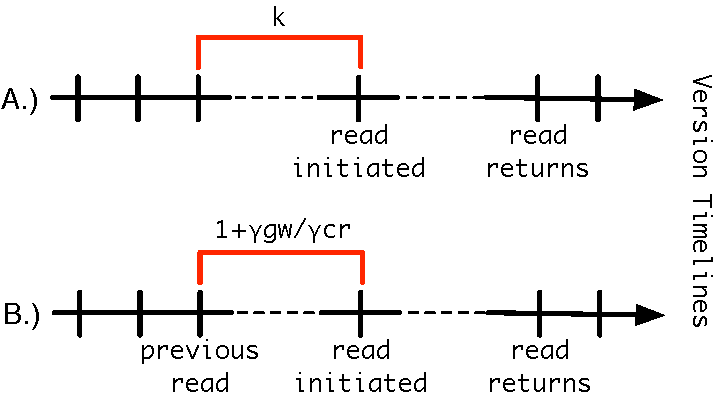
\includegraphics[width=.95\columnwidth]{figs/timelines.pdf}
\vspace{-8pt}
\caption{Versions returnable by read operations under PBS
  $k$-staleness (A) and PBS monotonic reads (B). In $k$-staleness, the
  read operation will return a version no later than $k$ versions
  older than the last committed value when it started.  In monotonic
  reads consistency, acceptable staleness depends on the number of
  versions committed since the client's last read.}
\vspace{-12pt}
\label{fig:timelines}
\end{figure}

The probability of returning a version of a key within the last $k$
versions committed is equivalent to intersecting one of $k$
independent write quorums.  Given the probability of a single quorum
non-intersection $p$, the probability of non-intersection with one of
the last $k$ independent quorums is $p^k$.  In our running example, the probability of non-intersection is Equation
\ref{eq:prob-strict} exponentiated by $k$:
\begin{equation}
\label{eq:k-consistency}
p_{sk} = \left(\frac{{N-W \choose R}}{{N \choose R}}\right)^k
\end{equation}

When $N$$=$$3$, $R$$=$$W$$=$$1$, this means that the probability of
returning a version within $2$ versions is $.\overline{5}$, within $3$
versions, $.\overline{703}$, $5$ versions, $> .868$, and $10$
versions, $>.98$.  When $N$$=$$3$, $R$$=$$1$, $W$$=$$2$ (equivalently,
$R$$=$$2$, $W$$=$$1$), these probabilities increase: $k$$=$$1
\rightarrow .\overline{6}$, $k$$=$$2 \rightarrow .\overline{8}$, and
$k$$=$$5 \rightarrow > .995$.

This closed form solution holds for quorums that do not change size
over time.  For expanding partial quorum systems, this solution is an
upper bound on the probability of staleness.  We discuss the
\textit{load} improvements offered by PBS $k$-staleness as discussed
in the quorum system literature i

\vspace{\subsectionskip}\subsection{PBS Monotonic Reads}

PBS $k$-staleness can be used to predict whether a client will ever
older staler data than it has already read, a well-known session
guarantee called \textit{monotonic reads}
consistency~\cite{sessionguarantees}.  This is particularly useful
when clients do not need to see the most recent version of a data item
but still require a notion of ``forward progress'' through versions,
as in timelines or streaming changelogs.

\begin{definition}
\label{def:prob-mr}
A quorum system obeys \textit{PBS monotonic reads consistency} if,
with probability at least $1-p_{sMR}$, at least one value in any
read quorum returned to a client is the same version or a newer
version than the last version that the client previously read.
\end{definition}

To guarantee that a client sees monotonically increasing versions, it
can continue to contact the same replica~\cite{vogels-defs} (provided
the ``sticky'' replica does not fail).  However, this is insufficient
for strict monotonic reads (where the client reads strictly newer data
if it exists in the system).  Definition~\ref{def:prob-mr} can be
adapted to accommodate strict monotonic reads by requiring that, if a
more recent data version is available, it is returned.

PBS monotonic reads consistency is a special case of PBS $k$-staleness
(see Figure~\ref{fig:timelines}B), where $k$ is determined by a
client's rate of reads from a data item ($\gamma_{cr}$) and the
global, system-wide rate of writes to the same data item
($\gamma_{gw}$).  If we know these rates, the number of
versions written between client reads is
$\frac{\gamma_{gw}}{\gamma_{cr}}$, as shown in Figure
\ref{fig:timelines}B.  We can calculate the probability of
probabilistic monotonic reads as a special case of $k$-staleness where
$k=1+\frac{\gamma_{gw}}{\gamma_{cr}}$.  Again extending our
running example, from Equation \ref{eq:k-consistency}:
\begin{equation}
\label{eq:prob-mr}
p_{sMR} = \left(\frac{{N-W \choose R}}{{N \choose R}}\right)^{1+\gamma_{gw}/\gamma_{cr}}
\end{equation}
For strict monotonic reads, where we cannot read the version we have
previously read (assuming there are newer versions in the database), we
exponentiate with $k=\frac{\gamma_{gw}}{\gamma_{cr}}$.

In practice, we may not know these exact rates, but, by measuring
their distribution, we can calculate an expected value.  By performing
appropriate admission control, operators can control these rates to
achieve monotonic reads consistency with high probability.

\subsection{Load Improvements}

Theory literature defines the \textit{load} of a quorum system as a
metric for the frequency of accessing the busiest quorum
member~\cite[Definition 3.2]{quorumsystems}.  Intuitively, the busiest
quorum member limits the number of requests that a given quorum system
can sustain, called its \textit{capacity}~\cite[Corollary
  3.9]{quorumsystems}.

Prior work determined that probabilistic quorum systems did not offer
significant benefits to load (providing a constant factor improvement
compared to strict quorum systems)~\cite{prob-quorum}.  Here, we show
that quorums tolerating PBS $k$-staleness have asymptotically lower
load than traditional probabilistic quorum systems (and, transitively,
than strict quorum systems).

The probabilistic quorum literature defines an
$\varepsilon$-intersecting quorum system as a quorum system that
provides a $1-\varepsilon$ probability of returning consistent
data~\cite[Definition 3.1]{prob-quorum}.  A $\varepsilon$-intersecting
quorum system has load of at least 
$\frac{1-\sqrt{\varepsilon}}{\sqrt{N}}$~\cite[Corollary
  3.12]{prob-quorum}.

In considering $k$ versions of staleness, we consider the intersection
of $k$ $\varepsilon$-intersecting quorum systems.  For a given
probability $p$ of inconsistency, if we are willing to tolerate $k$
versions of staleness, we need only require that that $\varepsilon =
\sqrt[k]{p}$.  This implies that our PBS $k$-staleness system
construction has load of at least
$\frac{(1-p)^{\frac{1}{2k}}}{\sqrt{N}}$, an improved lower bound
compared to traditional probabilistic quorum systems.  PBS monotonic
reads consistency results in a lower bound on load of
$\frac{(1-p)^{\frac{1}{2C}}}{\sqrt{N}}$, where
$C=1+\frac{\gamma_{gw}}{\gamma_{cr}}$.

These results are intuitive: if we are willing to tolerate multiple
versions of staleness, we need to contact fewer replicas.  Staleness
tolerance lowers the load of a quorum system, subsequently increasing
its capacity.

\vspace{\subsectionskip}\subsection{PBS $t$-visibility}
\label{sec:tvis}

Until now, we have considered only quorums that do not grow over time.
However, as we discussed in Section \ref{sec:practice}, real-world
quorum systems expand by asynchronously propagating writes to quorum
system members over time.  This process is commonly known as
anti-entropy~\cite{antientropy}.  For generality, in this section, we
will discuss generic anti-entropy. However, we explicitly model the
Dynamo-style anti-entropy mechanisms in Section \ref{sec:dynamo}.

PBS $t$-visibility models the probability of inconsistency for
expanding quorums.  Intuitively, PBS $t$-visibility captures the
possibility that a reader will observe a write $t$ seconds after it
commits. This captures the expected length of a ``window of
inconsistency'' resulting from partial quorum operation.  Recall that
we consider in-flight writes---which are more recent than the last
committed version---as non-stale.

\begin{definition}
A quorum system obeys \textit{PBS $t$-visibility consistency} if, with
probability $1-p_{st}$, any read quorum started at least $t$ units
of time after a write commits returns at least one value
that is at least as recent as that write.
\end{definition}

Overwriting data items effectively resets $t$-visibility;
$t$-visibility time is bounded by the time between writes.
Intuitively, if two writes to a key are spaced $m$ milliseconds apart,
then the $t$-visibility of the first write for $t > m$ milliseconds is
undefined; after $m$ milliseconds, there will be a newer version.

We denote the cumulative density function describing the number of
replicas $\mathcal{W}_r$ that have received a particular version $v$
exactly $t$ seconds after $v$ commits as $P_w(\mathcal{W}_r, t)$.

By definition, for expanding quorums, $\forall c \in [0, W], P_w(c,0)
= 1$; at commit time, $W$ replicas will have received the value with
certainty.  We can model the probability of PBS $t$-visibility for given $t$ by summing the conditional probabilities of each possible
$\mathcal{W}_r$:
\begin{equation}
\label{eq:tv-instantreads}
p_{st} = \frac{{N-W \choose N}}{{N \choose R}}+\sum_{c\in(W, N]} \frac{{N-c \choose N}}{{N \choose R}}\cdot [P_w(c+1, t)-P_w(c,t)]
\end{equation}
However, the above equation assumes reads occur instantaneously and
writes commit immediately after $W$ replicas have the version (i.e.,
there is no delay acknowledging the write to the coordinating node).
In the real world, writes need to be acknowledged and read requests
take time to arrive at remote replicas, increasing $t$.  Accordingly,
Equation~\ref{eq:tv-instantreads} is a conservative upper bound on
$p_{st}$.

In practice, $P_w$ depends on the anti-entropy mechanisms in use and
the expected latency of operations but can be approximated (Section
\ref{sec:dynamo}) or measured online.  For this reason, the load of a
PBS $t$-visible quorum system depends on write propagation and is
difficult to analytically determine for general-purpose expanding
quorums.  Additionally, one can model both transient and permanent
failures by increasing the tail probabilities of $P_w$
(Section~\ref{sec:discussion}).


\vspace{\subsectionskip}\subsection{PBS $\langle k, t \rangle$-staleness}

We can combine the previous models to combine both versioned and
real-time staleness metrics to determine the probability that a read
will return a value no older than $k$ versions stale if the last write
committed at least $t$ seconds ago:
\begin{definition}
A quorum system obeys \textit{PBS $\langle k, t \rangle$-staleness
  consistency} if, with probability $1-p_{skt}$, at least one value in
any read quorum will be within $k$ versions of the latest committed
version when the read begins, provided the read begins $t$ units of
time after the previous $k$ versions commit.
\end{definition}
The definition of $p_{skt}$ follows from the prior definitions:
\begin{equation}
p_{skt} = (\frac{{N-W \choose R}}{{N \choose R}}+\sum_{c\in[W, N)} \frac{{N-c \choose R}}{{N \choose R}} \cdot [P_w(c+1, t)-P_w(c,t)])^k
\end{equation}
In this equation, in addition to (again) assuming instantaneous reads,
we also assume the pathological case where the last $k$ writes all
occurred at the same time.  If we can determine the time since commit
for the last $k$ writes, we can improve this bound by considering each
quorum's $p_{skt}$ separately (individual $t$).  However, predicting
(and enforcing) write arrival rates is challenging and may introduce
inaccuracy, so this equation is a conservative upper bound on
$p_{skt}$.

Note that the prior definitions of consistency are encapsulated by PBS
$\langle k, t \rangle$-staleness consistency. Probabilistic $k$-quorum
consistency is simply PBS $\langle k, 0 \rangle$-staleness consistency,
PBS monotonic reads consistency is $\langle
1+\frac{\gamma_{gw}}{\gamma_{cr}}, 0 \rangle$-staleness consistency, and
PBS $t$-visibility is $\langle 1, t \rangle$-staleness consistency.

In practice, we believe it is easier to reason about staleness of
versions or staleness of time but not both together.  Accordingly,
having derived a closed-form model for $k$-staleness, in the remainder
of this paper, we focus mainly on deriving more specific models for
$t$-visibility. A conservative rule-of-thumb going forward is to
exponentiate the probability of inconsistency in $t$-visibility by $k$
when up to $k$ versions of staleness are tolerable.

\vspace{\sectionskip}\section{Dynamo-style $t$-visibility}
\label{sec:dynamo}

We have a closed-form model for $k$-staleness, but
$t$-visibility is dependent on both the quorum replication algorithm
and the anti-entropy processes employed by a given system.  In this
section, we discuss PBS $t$-visibility in the context of Dynamo-style
data storage systems and describe how to asynchronously detect
staleness.

\vspace{\subsectionskip}\subsection{Inconsistency in Dynamo: {\large \textit{WARS}} Model}
\label{sec:wars}

Dynamo-style quorum systems are inconsistent as a result of read and
write message reordering, a product of message delays.  Reads and
writes are sent to all quorum members, so the staleness under normal
operation results only when all of the first $R$ responses to a read
request arrived at their respective replicas before the last committed
write request.  To illustrate this phenomenon, we introduce a model
of message latency in Dynamo operation which, for convenience, we will
call \textit{WARS}.

In Figure~\ref{fig:dynamo-diagram}, we illustrate \textit{WARS} using
a space-time diagram for messages between a coordinator and a single
replica for a write followed by a read $t$ seconds after the write
commits.  This $t$ corresponds to the $t$ in PBS $t$-visibility.

\begin{figure}
\centering
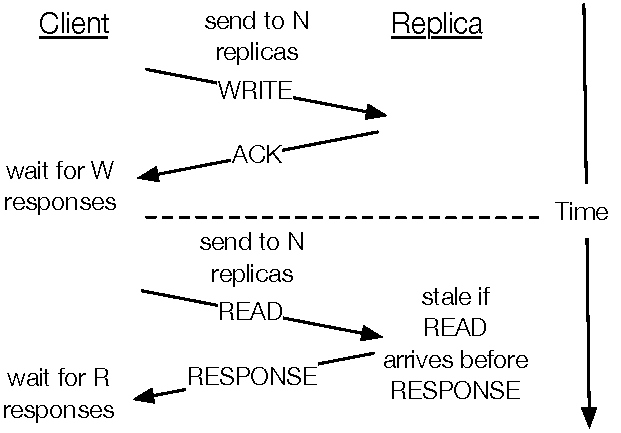
\includegraphics[width=.8\columnwidth]{figs/dynamostale.pdf}
\vspace{-8pt}
\caption{The \textit{WARS} model for in Dynamo describes the message
  latencies between a coordinator and a single replica for a write
  followed by a read $t$ seconds after commit.  In an $N$ replica
  system, this messaging occurs $N$ times.}
\vspace{-12pt}
\label{fig:dynamo-diagram}
\end{figure}

For a write, the coordinator sends $N$ messages, one to each
replica. The message from coordinator to replica containing the
version to be written is delayed by a value chosen from distribution
\texttt{W}.  The coordinator waits for $W$ responses from the replicas
before it can consider the version committed.  Each response
acknowledging the write is delayed by a value chosen from the
distribution \texttt{A}.

For a read, the coordinator (possibly different than the write
coordinator) sends $N$ messages, one to each replica.  The message
from coordinator to replica containing the read request is delayed by
a value chosen from distribution \texttt{R}.  The coordinator waits
for $R$ responses from the replicas before returning the most recent
value it receives.  The read response from each replica is delayed by
a value chosen from the distribution \texttt{S}.

The read coordinator will return stale data if the first $R$ responses
received reached their respective replicas before the replicas
received the latest version (delayed by \texttt{W}).  When
$R$$+$$W$$>$$N$, this is impossible.  However, under partial quorums,
the frequency of this occurrence depends on the latency distributions.
If we denote the commit time (when the coordinator has recieved $W$
acknowledgments) as $w_t$, a single replica's response is stale if
$r'+w_t+t< w'$ for $r'$ chosen from \texttt{R} and $w'$ chosen from
\texttt{W}.  Writes have time to propagate to additional replicas both
while the coordinator waits for all required acknowledgments
(\texttt{A}) and as read requests are sent (\texttt{R}).  Read
responses are further delayed in transit (\texttt{S}) back to the read
coordinator, inducing further possibility of reordering.
Qualitatively, longer write tails (\texttt{W}) and faster reads
increase the chance of staleness due to reordering.

\textit{WARS} considers the effect of message sending, delays, and
reception, but this represents a daunting analytical formulation.  The
commit time is an order statistic of $W$ and $N$ dependent on both
\texttt{W} and \texttt{A}.  Furthermore, the probability that the
$i$th returned read message observes reordering is another order
statistic of $R$ and $N$ dependent on
\texttt{W},\texttt{A},\texttt{R}, and \texttt{S}.  Moreover, across
responses, the probabilities are dependent. These dependencies make
calculating the probability of staleness rather difficult.  Dynamo is
straightforward to reason about and program but is difficult to
analyze in a simple closed form, which eludes us.  As we discuss in
Section~\ref{sec:mcsim}, we instead explore \textit{WARS} using Monte
Carlo methods, which are straightforward to understand and implement.

\vspace{\subsectionskip}\subsection{{\large \textit{WARS}} Scope}
\label{sec:anti-entropy}

\textbf{Proxying operations.} Depending on which coordinator a client
contacts, some reads and writes may be served locally.  In this case,
subject to local query processing delays, a read or write to $R$ or
$W$ nodes behaves like a read or write to $R-1$ or $W-1$ nodes,
respectively.  Although we do not do so, \textit{WARS} can be adopted
to handle local reads and writes.  Determining whether requests will
be proxied (and, if not, which replicas serve which requests) is data
store and deployment-specific.  Dynamo forwards write requests to a
designated coordinator solely for the purpose of establishing a
version ordering~\cite[Section 6.4]{dynamo} (easily achievable through
other mechanisms~\cite{zookeeper}).  Dynamo's authors observed a
latency improvement by proxying all operations and having clients act
as coordinators---Voldemort adopts this
architecture~\cite{voldemortclient}.

\textbf{Client-side delays.} Many end-users will incur additional time
between their respective reads and writes due to latency required to
contact the service.  Individuals making requests to web services
through their browsers will likely space sequential requests by tens
or hundreds of milliseconds due to client-to-server latency.  Although
we do not consider this delay here, it is important to remember for
practical scenarios because the delay between reads and writes ($t$)
may be large.

\textbf{Additional anti-entropy.} As we discussed in
Section~\ref{sec:practice}, anti-entropy decreases the probability of
staleness by further propagating versions between members.
Dynamo-style systems also support additional anti-entropy
processes~\cite{nosql}.  One common process is called \textit{read
  repair}: when a read coordinator receives multiple versions of a
data item from different replicas in response to a read request, it
will attempt to (asynchronously) update the out-of-date replicas with
the most recent version~\cite[Section 5]{dynamo}.  Read repair acts
like an additional write for every read, except old values are
re-written.  Additionally, Dynamo used Merkle trees to summarize and
exchange data contents between replicas~\cite[Section 4.7]{dynamo}.
However, not all Dynamo-style data stores actively employ similar
gossip-based anti-entropy.  For example, Cassandra uses Merkle tree
anti-entropy only when it is manually requested (e.g., \texttt{nodetool
  repair}), choosing to rely primarily on quorum expansion and read
repair~\cite{cassandra-merkle}.

These processes are rate-dependent: read repair's efficiency depends
on the rate of reads, and Merkle tree exchange's efficiency (and, more
generally, most anti-entropy efficiency) depends on the rate of
exchange.  A conservative assumption for read repair and Merkle tree
exchange is that they never occur. For example, assuming a particular
read repair rate implies a given rate of reads from each key in the
system.  \textit{WARS} only captures expanding quorum behavior but is
read rate independent and makes conservative assumptions about the
write rate.  If multiple writes overlap (that is, have overlapping
periods where they are in-flight but are not committed) the
probability of inconsistency decreases.  This is because
overlapping writes result in an increased chance that a client reads
as-yet-uncommitted data.  Versions may be fresher than
predicted.\begin{comment} {\color{red} Peter A: more
    general}\end{comment}

\vspace{\subsectionskip}\subsection{Asynchronous Staleness Detection}

Even if a system provides a low probability of inconsistency,
applications may need to be notified when data returned is
inconsistent or staler than expected.  Here, as a side note, we
discuss how the Dynamo protocol is naturally equipped for staleness
detection.  The following discussion is couched in the terms of PBS
$t$-visibility but is easily extended to PBS $k$-staleness and
$\langle k, t \rangle$-staleness.

Knowing whether a response is stale at read time requires strong
consistency.  Intuitively, by checking all possible values in the domain against a
hypothetical staleness detector, we could determine the (strongly) consistent
value to return.  While we cannot do so synchronously, we \textit{can}
determine staleness asynchronously.  Asynchronous staleness detection
allows speculative execution~\cite{nsdispeculation} if a program
contains appropriate compensation logic.

We first consider a staleness detector providing false positives.
Recall that, in a Dynamo-style system, we wait for $R$ of $N$ replies
before returning a value.  The remaining $N-R$ replicas will still
reply to the read coordinator.  Instead of dropping these messages,
the coordinator can compare them to the version it returned.  If there
is a mismatch, then either the coordinator returned stale data, there
are in-flight writes in the system, or additional versions committed
after the read. The latter two cases, relating to data committed after
the response was initiated, lead to false positives.  In these cases,
the read did not return ``stale'' data even though there were newer
but uncommitted versions in the system.  Notifying clients about newer
but uncommitted versions of a data item is not necessarily bad but may
be unnecessary and violates our staleness semantics.  This detector
does not require modifications to the Dynamo protocol and is similar
to the read-repair process.

To eliminate these uncommitted-but-newer false positives (cases two
and three), we need to determine the total, system-wide commit
ordering of writes. Recall that replicas are unaware of the commit
time for each version. The timestamps stored by replicas are not
updated after commit, and commits occur after $W$ replicas
respond. Thankfully, establishing a total ordering among distributed
agents is a well-known problem that could be accomplished in Dynamo
using a centralized service~\cite{zookeeper} or using distributed
consensus~\cite{paxos}. This requires modifications but is feasible.



\vspace{\sectionskip}\section{Evaluating Dynamo {\large $t$}-visibility}
\label{sec:dynamoeval}

As discussed in Section~\ref{sec:tvis}, PBS $t$-visibility depends on
the propagation of reads and writes throughout a system.  We
introduced the \textit{WARS} model as a means of reasoning about
inconsistency in Dynamo-style quorum systems, but quantitative metrics
such as staleness observed in practice depend on each of
\textit{WARS}'s latency distributions.  In this section, we perform an
analysis of Dynamo-style $t$-visibility to better understand how
frequently ``eventually consistent'' means ``consistent'' and, more
importantly, why.

PBS $k$-staleness is easily captured in closed form
(Section~\ref{sec:kstale}).  It does not depend on write latency or
any environmental variables.  Indeed, in practice, without expanding
quorums or anti-entropy, we observe that our derived equations hold
true experimentally.

$t$-visibility depends on anti-entropy, which is substantially more
complicated.  In this section, we focus on deriving experimental
expectations for PBS $t$-visibility.  While we could improve the
staleness results by considering additional anti-entropy processes
(Section~\ref{sec:anti-entropy}), we make the bare minimum of
assumptions required by the \textit{WARS} model.  Conservative
analysis decreases the number of experimental variables (supported by
empirical observations from practitioners) and increases the
applicability of our results.

\vspace{\subsectionskip}\subsection{Monte Carlo Simulation}
\label{sec:mcsim}

In light of the complicated analytical formulation discussed in
Section~\ref{sec:wars}, we implemented \textit{WARS} in an
event-driven simulator for use in Monte Carlo methods.  Calculating
$t$-visibility for a given value of $t$ is straightforward. Denoting the
$i$th sample drawn from distribution \texttt{D} as $\texttt{D}[i]$:
draw $N$ samples from \texttt{W}, \texttt{A}, \texttt{R}, and
\texttt{S} at time $t$, compute $w_t$, the $W$th smallest value of $\{\texttt{W}[i]+\texttt{A}[i], i \in [0, N)\}$, and check whether the first
$R$ samples of \texttt{R}, ordered by $\texttt{R}[i]+\texttt{S}[i]$
obey $w_t+\texttt{R}[i] + t\leq \texttt{W}[i]$.  This requires only a
few lines of code.  Extending this formulation to analyze $\langle k,
t \rangle$-staleness given a distribution of write arrival times
requires accounting for multiple writes across time but is not
difficult.

\subsection{Experimental Validation}

To validate \textit{WARS}, our simulator, and our subsequent analyses,
we compared our predicted $t$-visibility and latency with measured
values observed in a commercially available, open source Dynamo-style
data store.  We modified Cassandra to profile \textit{WARS} latencies,
disabled read repair (as it is external to \textit{WARS}), and, for
reads, only considered the first $R$ responses (often, more than $R$
messages would arrive by the processing stage, decreasing staleness).
We ran Cassandra on three servers with 2.2GHz AMD Opteron 2214
dual-core SMT processors and 4GB of 667MHz DDR2 memory, serving
in-memory data.  To measure staleness, we inserted monotonically
increasing versions of a key while concurrently issuing read requests.
Solely for the purpose of validation across several conditions, we
injected latencies into Cassandra's messaging.

Our observations matched the \textit{WARS} predictions. We injected
each combination of exponentially distributed $\texttt{W}=\lambda \in
\{0.05,$ $0.1,$ $0.2\}$ (respective means $20$ms, $10$ms and $5$ms)
and $\texttt{A}$$=$$\texttt{R}$$=$$\texttt{S}=\lambda \in \{0.1,$
$0.2,$ $0.5\}$ (respective means $10$ms, $5$ms and $2$ms) across
50,000 writes.  After empirically measuring the \textit{WARS}
distributions, consistency, and latency for each partial quorum
configuration, we predicted the $t$-visibility and latency. Our
average $t$-visibility prediction RMSE was $0.28\%$
(std. dev. $0.05\%$, max. $0.53\%$) for each
$t\in$$\{1,$$\dots,$$199\}$ ms. Our predicted latency (for each of the
$\{1.0, \dots, 99.9$th$\}$ percentiles for each configuration) had an
average N-RMSE of $0.48\%$ (std. dev. $0.18\%$, max. $0.90\%$).  This
validates our Monte Carlo simulator.


\vspace{\subsectionskip}\subsection{Write Latency Distribution Effects}
\label{sec:synthetic}

As discussed in Section~\ref{sec:wars}, the \textit{WARS} model of
Dynamo-style systems dictates that high one-way write variance
(\texttt{W}) increases staleness.  To quantify these effects, we swept
a range of exponentially distributed write distributions (changing
parameter $\lambda$, which dictates the mean and tail of the
distribution) while fixing \texttt{A}=\texttt{R}=\texttt{S}.

Our results, shown in Figure~\ref{fig:varydelay}, confirm this
relationship.  When the variance of \texttt{W} is $0.0625$ms
($\lambda=4$, mean $.25$ms, one-fourth the mean of
\texttt{A}=\texttt{R}=\texttt{S}), we observe a $94\%$ chance of
consistency immediately after the write and $99.9\%$ chance after 1ms.
However, when the variance of \texttt{W} is $100$ms ($\lambda=.1$,
mean $10$ms, ten times the mean of \texttt{A}=\texttt{R}=\texttt{S}),
we observe a $41\%$ chance of consistency immediately after write and
a $99.9\%$ chance of consistency only after $65$ms.  As the variance
and mean increase, so does the probability of inconsistency.  Under
distributions with fixed means and variable variances (uniform,
normal), we observe that the mean of \texttt{W} is less important than
its variance if \texttt{W} is strictly greater than
\texttt{A}=\texttt{R}=\texttt{S}.

Decreasing the mean and variance of \texttt{W} improves the
probability of consistent reads.  This means that, as we will see,
techniques that lower one-way write latency result in lower
$t$-visibility.  Instead of increasing read and write quorum sizes,
operators could chose to lower (relative) \texttt{W} latencies through
hardware configuration or by delaying reads.  This latter option is
potentially detrimental to performance for read-dominated workloads and
may introduce undesirable queuing effects.

\begin{figure}
\centering
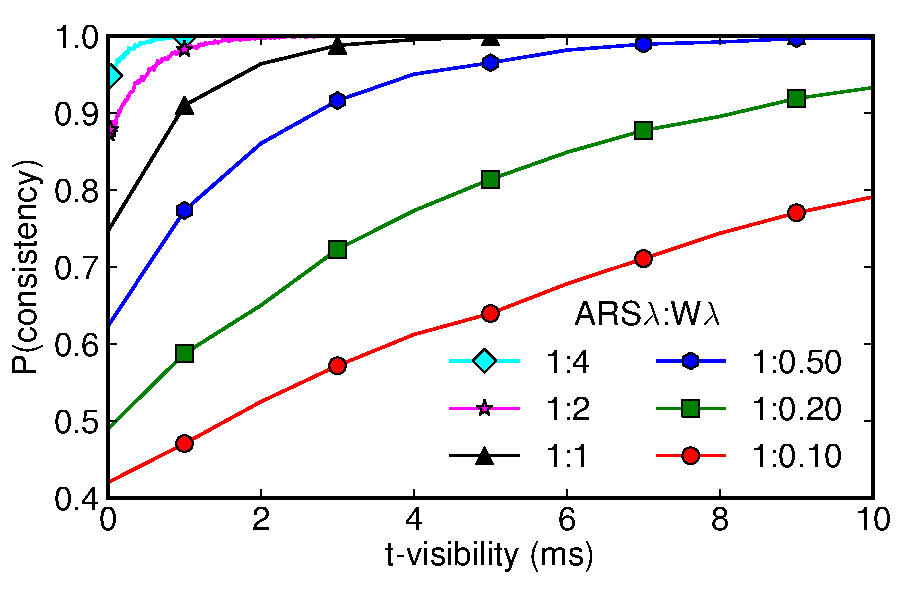
\includegraphics[width=.85\columnwidth]{figs/rwratio.pdf}
\vspace{-14pt}
\caption{$t$-visibility with
  exponential latency distributions for 
  \texttt{W} and \texttt{A}=\texttt{R}=\texttt{S}. Mean latency is
  $1/\lambda$. $N$$=$$3$, $R$$=$$W$$=$$1$. }
\vspace{-12pt}
\label{fig:varydelay}
\end{figure}

\vspace{\subsectionskip}\subsection{Production Latency Distributions}
\label{sec:latencies}

To study \textit{WARS} in greater detail, we obtained production latency
statistics from two internet-scale companies.

LinkedIn\footnote{LinkedIn. \url{www.linkedin.com}} is an online
professional social network with over 135 million members as of
November 2011. To provide highly available, low latency data storage,
engineers at LinkedIn built Voldemort.  Alex Feinberg, a lead engineer
on Voldemort, graciously provided us with latency distributions for a
single node under peak traffic for a user-facing service at
LinkedIn, representing 60\% read and 40\% read-modify-write
traffic~\cite{feinbergpc} (Table~\ref{table:linkedin}).  Feinberg
reports that, using spinning disks, Voldemort is ``largely IO bound
and latency is largely determined by the kind of disks we're using,
[the] data to memory ratio and request distribution.''  With solid-
state drives (SSDs), Voldemort is ``CPU and/or network bound
(depending on value size).''  As an aside, Feinberg also
noted that ``maximum latency is generally determined by [garbage
  collection] activity (rare, but happens occasionally) and is within
hundreds of milliseconds.''

\begin{table}
\centering
\begin{tabular}{|c|c|}
\hline
\%ile & Latency (ms) \\
\hline
\multicolumn{2}{|c|}{ 15,000 RPM SAS Disk}\\
\hline
Average & 4.85\\
95 & 15\\
99 & 25\\
\hline
\multicolumn{2}{|c|}{ Commodity SSD }\\
\hline
Average & 0.58 \\
95 & 1\\
99 & 2\\
\hline
\end{tabular}
\vspace{-6pt}
\caption{LinkedIn Voldemort single-node production latencies.}
\vspace{-4pt}
\label{table:linkedin}
\end{table}

Yammer\footnote{Yammer. \url{www.yammer.com}} is an online, private
social networking to over 100,000 companies as of December 2011 that
uses Basho's Riak for some client data~\cite{riak}.  Coda Hale, an
infrastructure architect, and Ryan Kennedy, also of Yammer, previously
presented in-depth performance and configuration details for their
Riak deployment in March 2011~\cite{riakyammer}.  Hale provided us
with more detailed performance statistics for their
application~\cite{codapc} (Table~\ref{table:yammer}).  Hale mentioned
that ``reads and writes have radically different expected latencies,
especially for Riak.''  Writes are delayed ``until the fsync returns,
so while reads are often $<$ 1ms, writes rarely are.''  Also, although
we do not model this explicitly, Hale also noted that the size of
values is important, claiming ``a big performance improvement by
adding LZF compression to values.''

\begin{table}
\centering
\begin{tabular}{|c|c|c|}
\hline
\%ile & Read Latency (ms) & Write Latency (ms)\\
\hline
Min & 1.55 & 1.68\\
50 & 3.75 & 5.73 \\
75 & 4.17 & 6.50\\
95 & 5.2 & 8.48\\
98 & 6.045 & 10.36 \\
99 & 6.59 & 131.73\\
99.9 & 32.89 & 435.83\\
Max & 2979.85 &  4465.28 \\
\hline
Mean & 9.23 & 8.62 \\
Std. Dev. & 83.93 & 26.10\\
\hline
Mean Rate & 718.18 gets/s & 45.65 puts/s\\
\hline
\end{tabular}
\vspace{-4pt}
\caption{Yammer Riak $N$$=$$3$, $R$$=$$2$, $W$$=$$2$ production latencies.}
\vspace{-12pt}
\label{table:yammer}
\end{table}

\subsection{Latency Model Fitting}

While the provided production latency distributions are invaluable,
they are under-specified for \textit{WARS}.  First, the data are
summary statistics, but \textit{WARS} requires distributions.  More
importantly, the provided latencies are round-trip times, while
\textit{WARS} requires the constituent one-way latencies for both
reads and writes.  As our validation demonstrated, these latency
distributions are easily collected, but, because they are not
currently collected in production, we must fill in the
gaps. Accordingly, to fit \texttt{W}, \texttt{A}, \texttt{R}, and
\texttt{S} for each configuration, we made a series of assumptions,
which we believe are justified given the benefit of production data.
Without additional data on the latency required to read multiple
replicas, we assume that each latency distribution is independently,
identically distributed (IID).  Each configuration fit a mixture model
with two separate distributions, one for the body and the other for
the tail.

LinkedIn provided two latency distributions, whose fits we denote
\texttt{LNKD-SSD} and \texttt{LNKD-DISK} for the SSD and spinning
disks, respectively.  As previously discussed, when running on SSDs,
Voldemort is largely network and CPU bound.  Accordingly, for
\texttt{LNKD-SSD}, we assumed that read and write operations took
equivalent amounts of time and, to allocate the remaining time, we
focused on the network-bound case and assumed that one-way messages
were symmetric (\texttt{W}=\texttt{A}=\texttt{R}=\texttt{S}). Feinberg
reported that Voldemort performs at least one read before every write
(average of 1 seek, between 1-3 seeks), and writes to the BerkeleyDB
Java Edition backend are flushed either every 30 seconds or 20
megabytes---whichever comes first~\cite{feinbergpc}.  Accordingly, for
\texttt{LNKD-DISK}, we used the same \texttt{A}=\texttt{R}=\texttt{S}
as \texttt{LNKD-SSD} but fit \texttt{W} separately.

Yammer provided distributions for a single configuration, denoted
\texttt{YMMR}, but separated read and write latencies.  Under our IID
assumptions, we fit single-node latency distributions to the provided
data, again assuming symmetric \texttt{A}, \texttt{R}, and \texttt{S}.
The data again fit a Pareto distribution with a long exponential tail.
At the $98$th percentile, the write distribution takes a sharp turn.
Fitting the data closely resulted in an extremely long tail, with
$99.99+$th percentile writes requiring tens of seconds---much higher
than Yammer specified.  Accordingly, we fit the $98$th percentile knee
conservatively; without the $98$th percentile, the write fit N-RMSE is
.104\%.

We also considered a wide-area network replication scenario, denoted
\texttt{WAN}.  Reads and writes originate in a random datacenter, and,
accordingly, one replica command completes quickly while the others
are routed remotely.  We delay remote operations and responses by 75ms
and apply \texttt{LNKD-DISK} delays once the command reaches a remote
data center, representing multi-continent WAN network
delay~\cite{dean-keynote}

We show the parameters for each distribution in
Table~\ref{table:fits} and plot each fitted distribution in
Figure~\ref{fig:latencies}.  Note that for $R$, $W$ of one,
\texttt{LNKD-DISK} is not equivalent to \texttt{WAN}.  This is
because, in \texttt{LNKD-DISK}, we only have to wait for the first of
$N$ local reads (writes) to return, whereas, for \texttt{WAN}, there
is only one local read (write) and all other read (write) requests are
delayed at least 150ms.


\begin{table}
\centering
\begin{tabular}{|c|r|}
\hline
\multirow{4}{*}{\texttt{LNKD-SSD}} & \multicolumn{1}{|l|}{$\texttt{W} = \texttt{A}= \texttt{R} = \texttt{S}:$} \\
& 91.22\%: Pareto, $x_m=.235, \alpha=10$\\
& 8.78\%: Exponential, $\lambda = 1.66$ \\
& N-RMSE: .55\%\\\hline
\multirow{4}{*}{\texttt{LNKD-DISK}} & 
 \multicolumn{1}{|l|}{\texttt{W}:}\\
& 38\%: Pareto, $x_m=1.05, \alpha=1.51$\\
& \hfill 62\%: Exponential, $\lambda = .183$ \\
& N-RMSE: .26\%\\\cline{2-2}
& \multicolumn{1}{|l|}{$\texttt{A}= \texttt{R} = \texttt{S}: \texttt{LNKD-SSD}$}\\
\hline
\multirow{8}{*}{\texttt{YMMR}} & \multicolumn{1}{|l|}{\texttt{W}:} \\
& 93.9\%: Pareto, $x_m=3, \alpha=3.35$\\
& 6.1\%: Exponential, $\lambda = .0028$ \\
& N-RMSE: 1.84\%\\\cline{2-2}
& \multicolumn{1}{|l|}{$\texttt{A}= \texttt{R} = \texttt{S}:$}\\
& 98.2\%: Pareto, $x_m=1.5, \alpha=3.8$\\
& 1.8\%: Exponential, $\lambda=.0217$\\
& N-RMSE: .06\%\\
\hline
\end{tabular}
\vspace{-6pt}
\caption{Distribution fits for production latency distributions from LinkedIn (\texttt{LNKD-*}) and Yammer (\texttt{YMMR}).}
\vspace{-12pt}
\label{table:fits}
\end{table}



\begin{figure*}[t!]
\centering
\subfigure{
\includegraphics[width=\columnwidth]{figs/latlegend.pdf}}\\[-1mm]
\subfigure{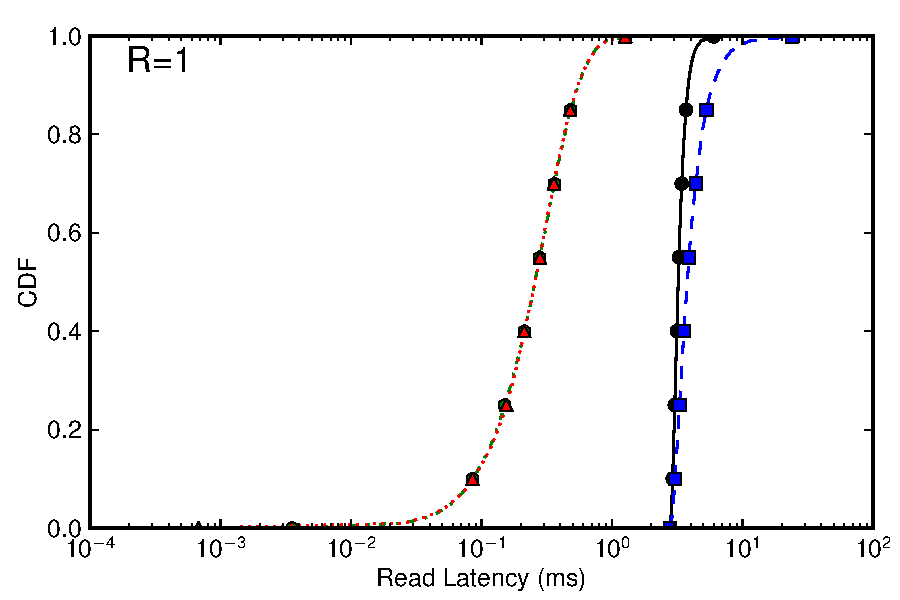
\includegraphics[width=.6\columnwidth]{figs/readlats-1.pdf}}
\subfigure{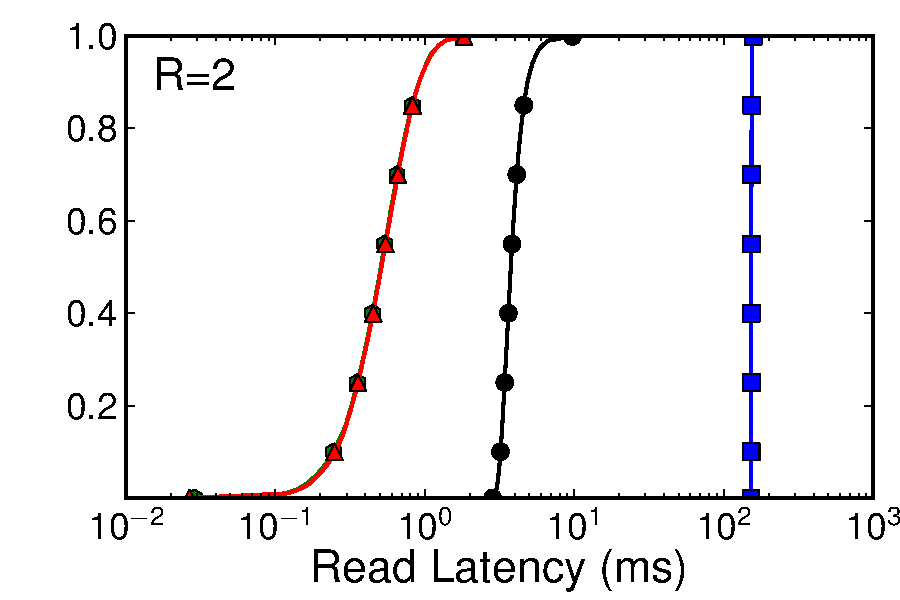
\includegraphics[width=.6\columnwidth]{figs/readlats-2.pdf}}
\subfigure{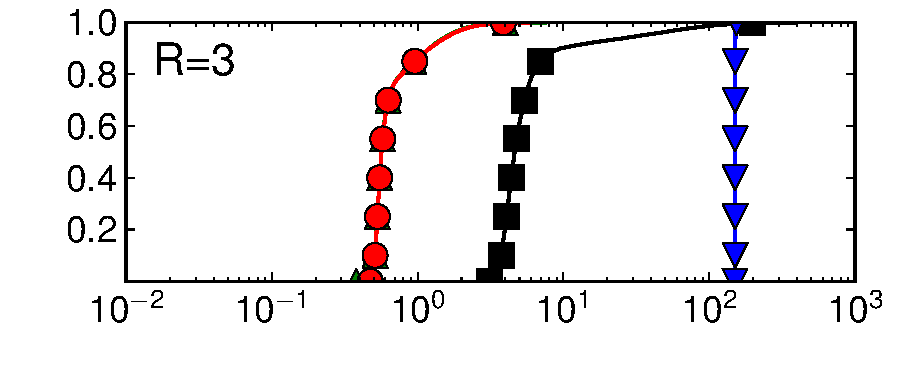
\includegraphics[width=.6\columnwidth]{figs/readlats-3.pdf}}
\subfigure{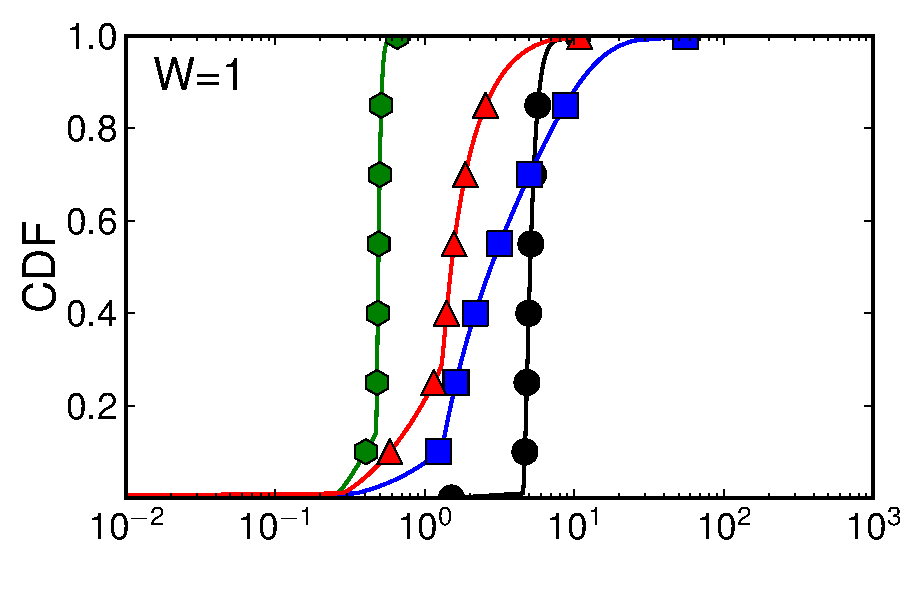
\includegraphics[width=.6\columnwidth]{figs/writelats-1.pdf}}
\subfigure{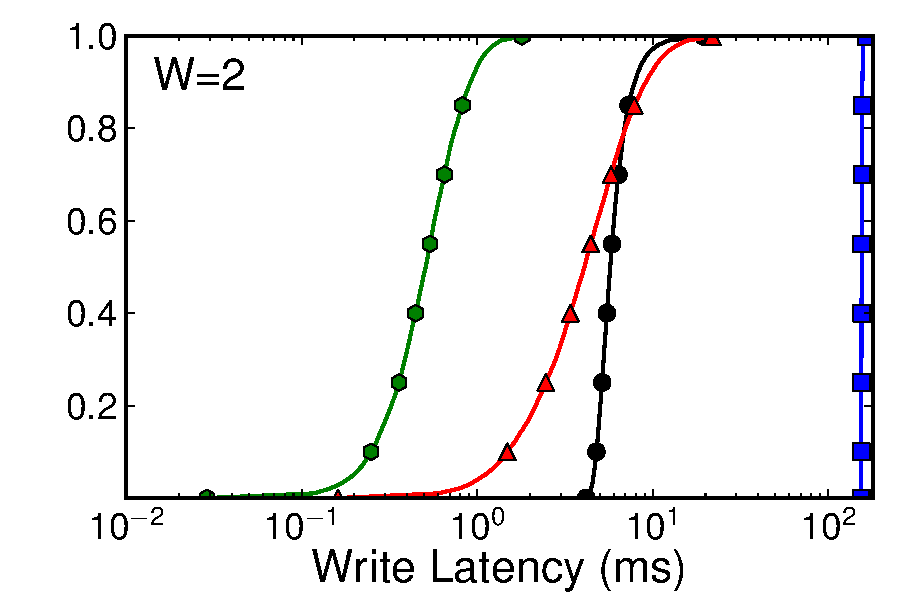
\includegraphics[width=.6\columnwidth]{figs/writelats-2.pdf}}
\subfigure{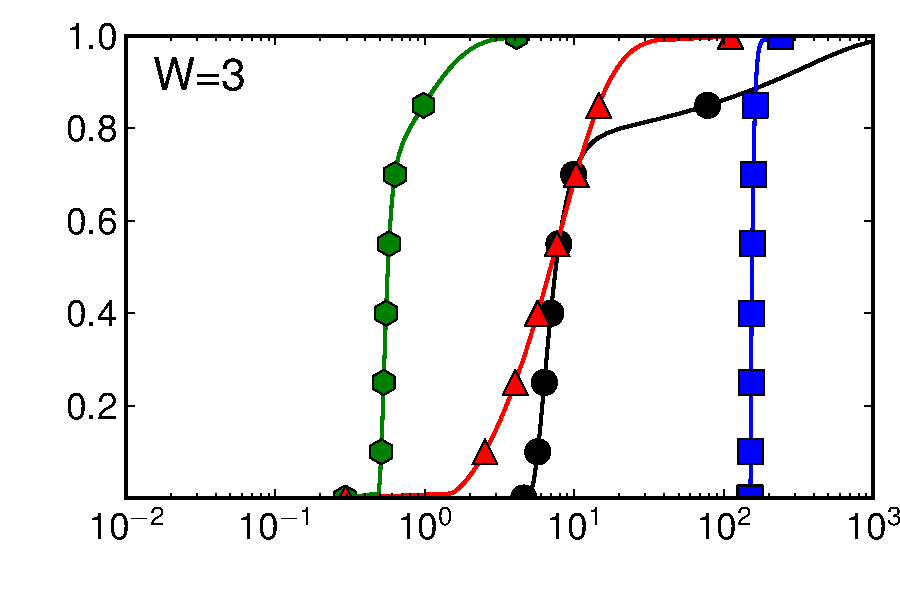
\includegraphics[width=.6\columnwidth]{figs/writelats-3.pdf}}
\vspace{-8pt}
\caption{Read and write operation latency for production fits for $N$$=$$3$. Note that, for reads, \texttt{LNKD-SSD} is equivalent to \texttt{LNKD-DISK}.}
\vspace{-8pt}
\label{fig:latencies}
\end{figure*}


\vspace{\subsectionskip}\subsection{Observed {\large$t$}-visibility}

We measured the $t$-visibility for each distribution
(Figure~\ref{fig:tvis}). As we observed under synthetic distributions
in Section~\ref{sec:synthetic}, the $t$-visibility depended on both
the relative mean and variance of \texttt{W}.

\texttt{LNKD-SSD} and \texttt{LNKD-DISK} demonstrate the importance of
write latency in practice.  Immediately after write commit,
\texttt{LNKD-SSD} had a $97.4\%$ probability of consistent reads,
reaching over a $99.999\%$ probability of consistent reads after five
milliseconds. \texttt{LNKD-SSD}'s reads briefly raced its writes
immediately after commit.  However, several milliseconds after the
write, the chance of a read arriving before the last write was almost
completely eliminated. The distribution's read and write operation
latencies were rather small (median $.489$ms), and writes completed
quickly across all replicas due to the distribution's short tail
($99.9$th percentile $.657$ms).  In contrast, under
\texttt{LNKD-DISK}, writes take significantly longer (median $1.50$ms)
and have a longer tail ($99.9$th percentile $10.47$ ms).  This
difference is reflected in its $t$-visibility: \texttt{LNKD-DISK} had
only a $43.9\%$ probability of consistent reads immediately after
write commit and only a $92.5\%$ probability ten milliseconds later.
This suggests that SSDs may drastically improve consistency in
practice due to reducing write variance.

We experienced similar effects with the other distributions.
Immediately after commit, \texttt{YMMR} had a $89.3\%$ chance of
consistency.  However, \texttt{YMMR}'s long tail hampered its
$t$-visibility increase and reached a $99.9\%$ probability of
consistency 1364 ms after commit.  As expected, \texttt{WAN} observed
poor chances of consistency until after the 75 milliseconds passed
($33\%$ chance immediately after commit); unless a client read from
the same datacenter in which the last write was issued, it had to wait
for the long propagation delay to observe the most recent value.

\begin{figure*}[t!]
\centering
\subfigure{
\includegraphics[width=.85\columnwidth]{figs/stalelegend.pdf}}\\[-1mm]
\subfigure{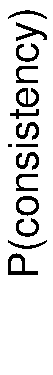
\includegraphics[width=3.2mm]{figs/staley.pdf}}
\subfigure{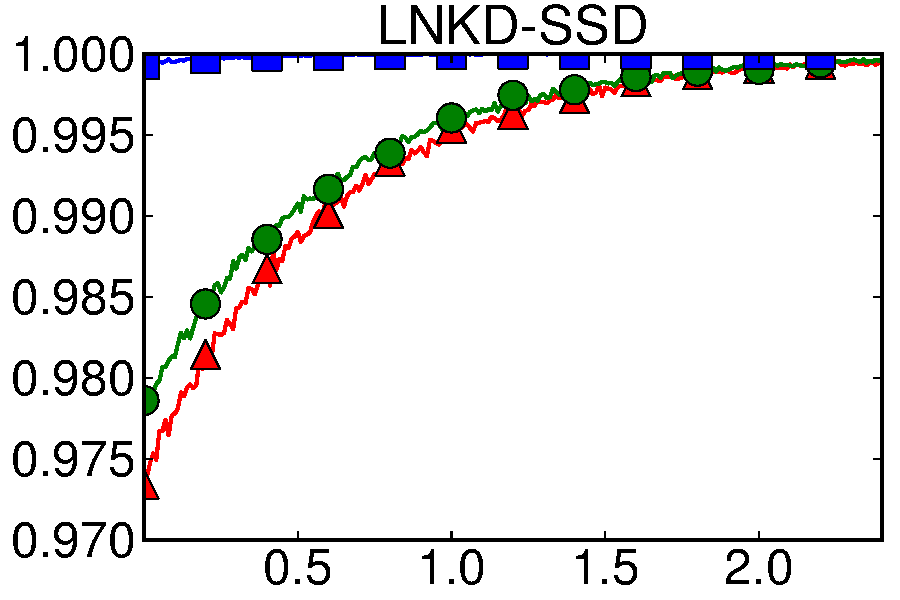
\includegraphics[width=.48\columnwidth]{figs/tstales-LNKD-SSD.pdf}}
\subfigure{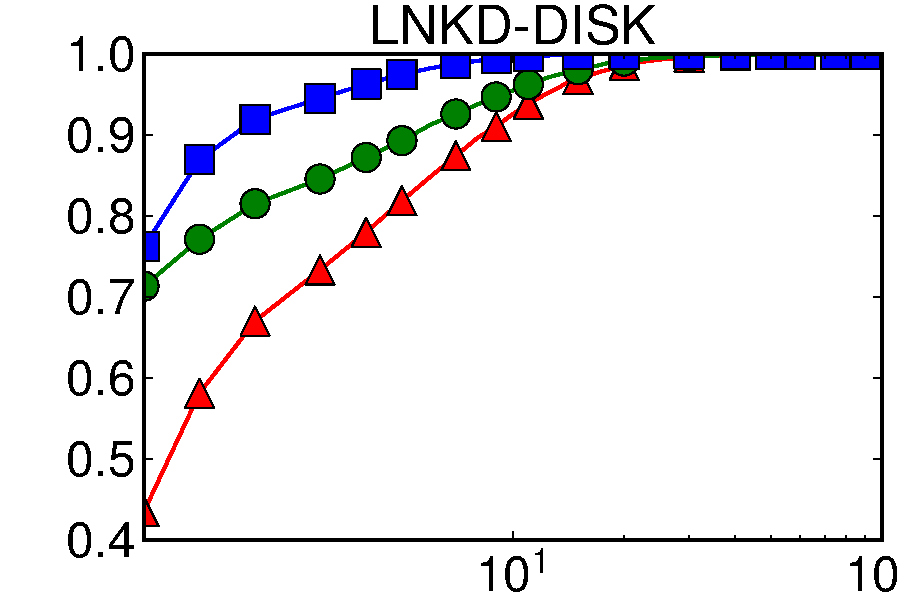
\includegraphics[width=.48\columnwidth]{figs/tstales-LNKD-DISK.pdf}}
\subfigure{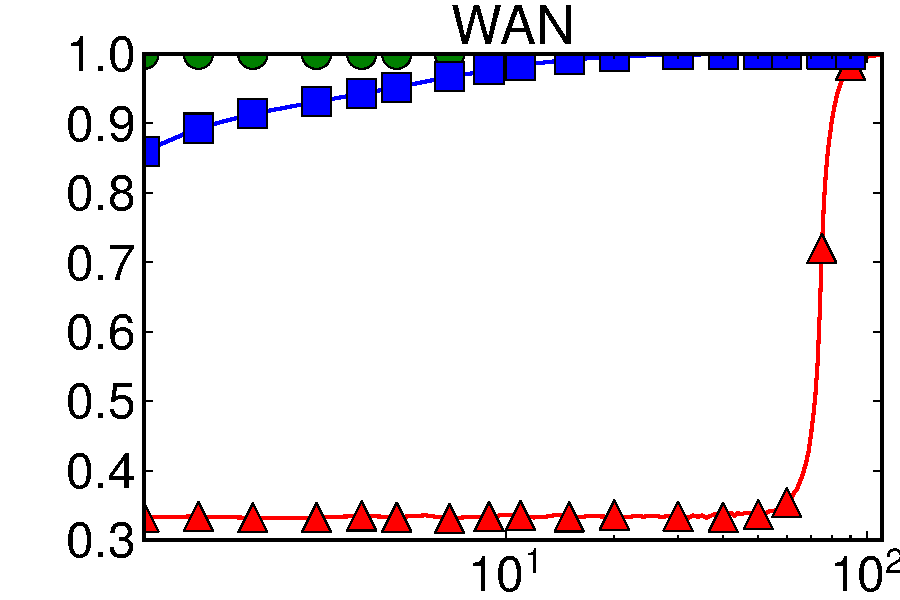
\includegraphics[width=.48\columnwidth]{figs/tstales-WAN.pdf}}
\subfigure{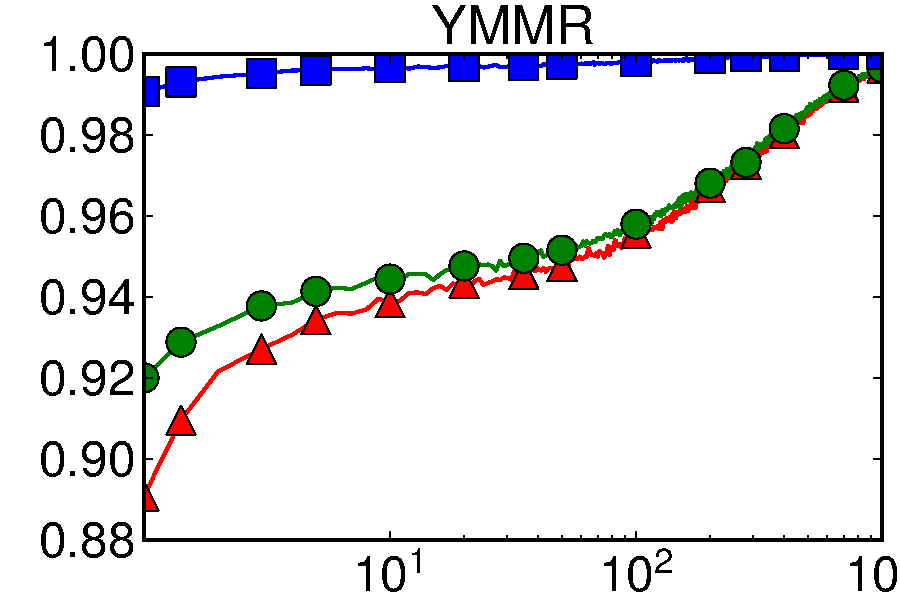
\includegraphics[width=.48\columnwidth]{figs/tstales-YMMR.pdf}}\\[-1mm]
\subfigure{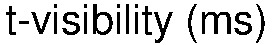
\includegraphics[width=17mm]{figs/stalex.pdf}}
\vspace{-10pt}
\caption{$t$-visibility for production operation latencies.}
\vspace{-6pt}

\label{fig:tvis}
\end{figure*}

\vspace{\subsectionskip}\subsection{Quorum Sizing}

In addition to $N$$=$$3$, we consider how varying the number of
replicas (N) affects $t$-visibility while maintaining
$R$$=$$W$$=$$1$. The results, depicted in Figure~\ref{fig:varyn}, show
that the probability of consistency immediately after write commit
decreases as $N$ increases.  With 2 replicas, \texttt{LNKD-DISK} has a
$57.5\%$ probability of consistent reads immediately after commit but
only a $21.1\%$ probability with 10 replicas.  However, at high
probabilities of consistency, the wait time required for increased
replica sizes is surprisingly close.  For \texttt{LNKD-DISK}, the
$t$-visibility at $99.9\%$ probability of consistency ranges from
$45.3$ms for 2 replicas to $53.7$ms for 10 replicas.

These results imply that maintaining a large number of replicas for
availability or better performance, results in a potentially large
impact on consistency immediately after writing. However, the
$t$-visibility staleness will still converge quickly.

\begin{figure*}[t!]
\centering
\subfigure{
\includegraphics[width=\columnwidth]{figs/nlegend.pdf}}\\[-1mm]
\subfigure{\includegraphics[width=.65\columnwidth]{figs/sweepn-LNKD-DISK.pdf}}
\subfigure{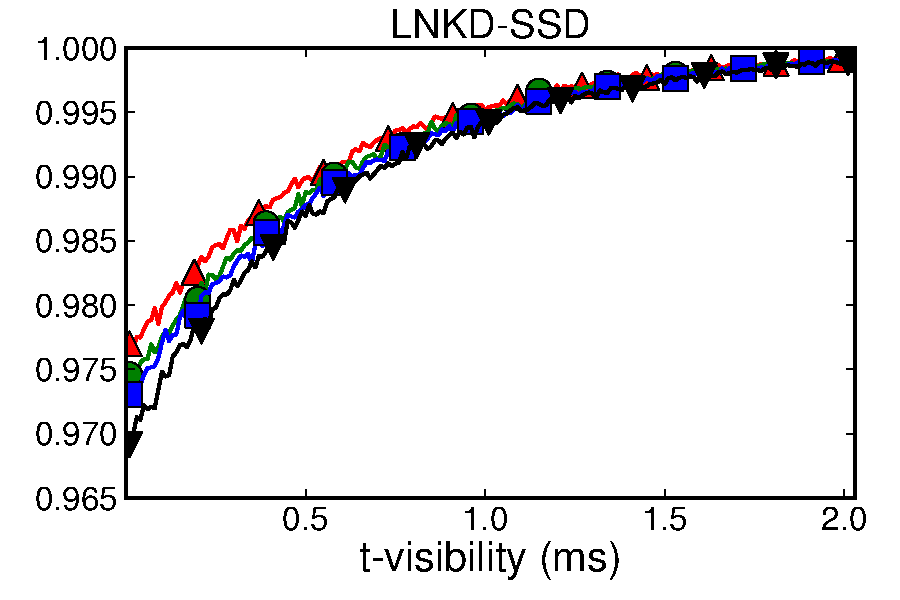
\includegraphics[width=.65\columnwidth]{figs/sweepn-LNKD-SSD.pdf}}
\subfigure{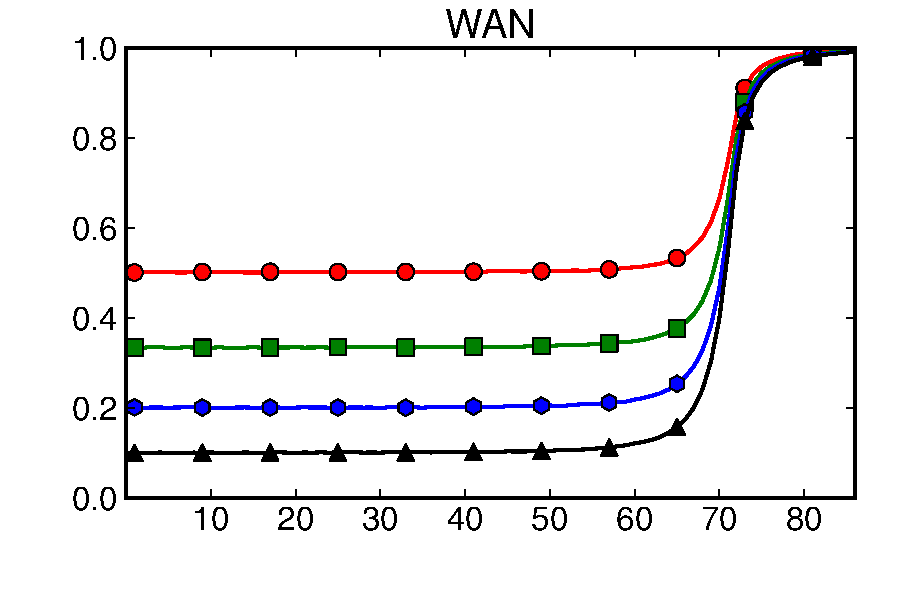
\includegraphics[width=.65\columnwidth]{figs/sweepn-WAN.pdf}}
\vspace{-14pt}
\caption{$t$-visibility for production operating latencies for variable $N$ and $R$$=$$W$$=$$1$.}
\vspace{-10pt}
\label{fig:varyn}
\end{figure*}

\vspace{\subsectionskip}\subsection{Latency vs. {\large $t$}-visibility}

Choosing a value for $R$ and $W$ is a trade-off between operation
latency and $t$-visibility. To measure the obtainable latency gains,
we compared $t$-visibility required for a $99.9\%$ probability of
consistent reads to the $99.9$th percentile read and write latencies.

Partial quorums can have a large impact on latency at a variable cost
to $t$-visibility (Table~\ref{table:lat-stale}).  For \texttt{YMMR},
$R$$=$$W$$=$$1$ results in low latency reads and writes ($16.4$ms) but
high $t$-visibility ($1364$ms). However, by setting $R$$=$$2$ and
$W$$=$$1$, we reduce $t$-visibility to $202$ms and the combined read
and write latencies are $81.1\%$ ($186.7$ms) lower than the fastest
strict quorum ($W$$=$$1$, $R$$=$$3$).  \texttt{LNKD-DISK} read and
write latencies can be reduced by $16.5\%$ ($2.48$ms) with
$t$-visibility of $13.6$ms.  The write tail of \texttt{LNKD-SSD} was
such that we never observed message reordering for $R$$=$$2$,
$W$$=$$1$, allowing a $30\%$ ($.98$ms) latency reduction with no
observable staleness (even across $10M$ writes, ``seven nines'').
$R$$=$$W$$=$$1$ reduced latency by $59.5\%$ ($1.94$ms) with a
corresponding $t$-visibility of $1.85$ms.  Under \texttt{WAN}, $R > 1$
or $W > 1$ results in a large latency increase because this requires
WAN messages. These results indicate that lowering values of $R$ and
$W$ can significantly improve operation latency and that
$t$-visibility can be low even when we require a high probability of
consistent reads.

\begin{table*}
\centering
\begin{tabular}{c|c|c|c|c|c|c|c|c|c|c|c|c|}
\cline{2-13}
 & \multicolumn{3}{|c|}{\texttt{LNKD-SSD}} & \multicolumn{3}{|c|}{\texttt{LNKD-DISK}} & \multicolumn{3}{|c|}{\texttt{YMMR}} & \multicolumn{3}{|c|}{\texttt{WAN}}\\
&\multicolumn{1}{|c}{$L_r$}  & \multicolumn{1}{c}{$L_w$} & \multicolumn{1}{c|}{$t$} &  \multicolumn{1}{|c}{$L_r$} & \multicolumn{1}{c}{$L_w$} & \multicolumn{1}{c|}{$t$} &  \multicolumn{1}{|c}{$L_r$} & \multicolumn{1}{c}{$L_w$} & \multicolumn{1}{c|}{$t$} &  \multicolumn{1}{|c}{$L_r$} & \multicolumn{1}{c}{$L_w$} & \multicolumn{1}{c|}{$t$} \\\hline
\multicolumn{1}{|c|}{$R$$=$$1$, $W$$=$$1$}
&  \textbf{0.66} & \textbf{0.66} & \textbf{1.85} & 0.66 & 10.99 & 45.5 & 5.58 & 10.83 & 1364.0 & \textbf{3.4} & \textbf{55.12} & \textbf{113.0} \\
\multicolumn{1}{|c|}{$R$$=$$1$, $W$$=$$2$}
&  0.66 & 1.63 & 1.79 & 0.65 & 20.97 & 43.3 & 5.61 & 427.12 & 1352.0 & 3.4 & 167.64 & 0 \\
\multicolumn{1}{|c|}{$R$$=$$2$, $W$$=$$1$}
& \textbf{1.63} & \textbf{0.65} & \textbf{0} & \textbf{1.63} & \textbf{10.9} & \textbf{13.6}& \textbf{32.6} & \textbf{10.73} & \textbf{202.0} & 151.3 & 56.36 & 30.2 \\
\multicolumn{1}{|c|}{$R$$=$$2$, $W$$=$$2$}
&  \textbf{1.62} & \textbf{1.64} & \textbf{0} & 1.64 & 20.96 & 0& 33.18 & 428.11 & 0 & 151.31 & 167.72 & 0 \\
\multicolumn{1}{|c|}{$R$$=$$3$, $W$$=$$1$}
&  4.14 & 0.65 & 0 & \textbf{4.12} & \textbf{10.89} & \textbf{0} & \textbf{219.27} & \textbf{10.79} & \textbf{0} & \textbf{153.86} & \textbf{55.19} & \textbf{0} \\
\multicolumn{1}{|c|}{$R$$=$$1$, $W$$=$$3$}
& 0.65 & 4.09 & 0 & 0.65 & 112.65 & 0& 5.63 & 1870.86 & 0 & 3.44 & 241.55 & 0 \\
\hline
\end{tabular}
\vspace{-4pt}
\caption{$t$-visibility for $p_{st} = .001$ ($99.9\%$ probability
  of consistency for $50,000$ reads and writes) and $99.9$th percentile read
  ($L_r$) and write latencies ($L_w$) across $R$ and $W$, $N$$=$$3$
  ($1M$ reads and writes). Significant latency-staleness trade-offs are in bold.}
\vspace{-12pt}
\label{table:lat-stale}
\end{table*}

\vspace{\sectionskip}\section{Discussion and Future Work}
\label{sec:discussion}

In this section, we discuss several enhancements to partial
quorum systems that PBS enables along with future work for PBS.

\textbf{Latency/Staleness SLAs.} With PBS, we can automatically
configure replication parameters by optimizing operation latency given
constraints on staleness and minimum durability.  Data store operators
can subsequently provide service level agreements to applications and
quantitatively describe latency/staleness trade-offs to users.
Operators can dynamically configure replication using online latency
measurements.  PBS provides a quantitative lens for analyzing
consistency guarantees that were previously unknown.  This
optimization formulation is likely non-convex, but the state space for
configurations is small ($O(N^2)$).  This optimization also allows
disentanglement of replication for reasons of durability from
replication for reasons of low latency and higher capacity.  For
example, operators can specify a minimum replication factor for
durability and availability but can also automatically increase
$N$, decreasing tail latency for fixed $R$ and $W$.

\textbf{Variable configurations.} We have assumed the use of a single
replica configuration ($N$, $R$, and $W$) across all operations.
However, one could vary these operations over time and across keys.
By specifying a target latency, one could periodically modify $R$ and
$W$ to more efficiently guarantee a desired bound on staleness, or
vice versa. These time-varying configurations require additional
refinements and revisit prior work on fluid
replication~\cite{fluidreplication}.

\textbf{Stronger guarantees.} We have focused on probabilistic
staleness analysis, but there is are many other, often stronger forms of eventual
consistency (such as causal consistency)~\cite{vogels-defs}.
Predicting the probability of attaining more complex consistency
semantics requires additional modeling of application access patterns.
This is possible, but we suspect that modeling the \textit{worst-case}
semantics of these operations will result in unfavorably low
probabilities of consistent operations.  We can see this in Aiyer et
al.'s analysis of Byzantine $k$-quorums~\cite{multi-k-quorum}: in a
worst-case deployment, with an adversarial scheduler, the lower bound
on guaranteed recency is quite high.  We conjecture that the bound
would be even higher had the authors performed an analysis of stronger
consistency models.

\textbf{Alternative architectures.} Dynamo is conceptually easy to
understand and implement (\textit{WARS}) but is painful to
analytically analyze.  Is there a design that finds a better middle
ground between operational elegance and simplicity of analysis within
the eventually consistent design space?  Prior work on deterministic
bounded staleness (Section~\ref{sec:relatedwork}) provides guidance
but often sacrifices availability and may be more complex to reason
about.

\textbf{Multi-key operations.} We have considered single-key
operations, however the ability to perform multi-key operations is
potentially attractive.  For read-only transactions, if the key
distribution is random and each quorum is independent, we can multiply
the staleness probabilities of each key to determine multi-key
staleness probabilities. Achieving atomicity of writes to multiple
keys requires more complicated coordination mechanisms such as
two-phase commit, increasing operation latency.  Transactions are
feasible but require considerable care in implementation, complicating
what is otherwise a simple replication scheme.

\textbf{Failure modes.} In our evaluation of $t$-visibility, we
focused on normal operating conditions. Unless failures are
common-case, they affect tail staleness probabilities (which appear as
latency spikes in \textit{WARS}).  For example, if, as Jeff Dean of
Google suggests~\cite{dean-keynote}, servers crash at least twice per
year, given a ten hour downtime per failure, this roughly represents
.23\% downtime per machine per year.  If failures are correlated, this
small percentage may be a problem. However, if they are independent, a
replica set of $N$ nodes with $F$ failed nodes behaves like an $N-F$
replica set.  The probability of all $N$ nodes failing is $(.23)^N$\%
(``five nines'' reliability for $N$$=$$3$) and will likely be hidden
in the probability tail.  Quantifying this impact more precisely would
be beneficial but requires additional information about failure rates
and their impact on latency distributions. Additionally, modeling
recovery semantics such as hinted handoff~\cite[Section 4.6]{dynamo}
would also be useful.

\vspace{\sectionskip}\section{Related Work}
\label{sec:relatedwork}

We surveyed quorum replication techniques~\cite{prob-quorum-dynamic,
  92-quorums, treequorum, non-strict, multi-k-quorum, quorums-start,
  quorum-placement, partitionedquorum, quorums-alternative,
  prob-quorum, quorum-overview, quorumsystems} in
Section~\ref{sec:background}.  In this work, we specifically draw
inspiration from probabilistic quorums~\cite{prob-quorum} and
deterministic $k$-quorums~\cite{ non-strict, multi-k-quorum} in
analyzing expanding quorum systems and their consistency.  We believe
that revisiting probabilistic quorum systems---including non-majority
quorum systems such as tree quorums---in the context of write
propagation, anti-entropy, and Dynamo is a promising area for
theoretical work.

Data consistency is a long-studied problem in distributed
systems~\cite{consistency-partitioned, danger-rep} and concurrent
programming~\cite{linearizability}.  Given the CAP Theorem and the
inability to maintain all three of consistency, availability, and
partition tolerance~\cite{cap-proof}, data systems have turned to
``eventually consistent'' semantics to provide availability in the
face of partitions~\cite{consistency-partitioning, vogels-defs}.
Real-time causal (RTC) consistency is the strongest consistency model
achievable in an available, one-way convergent (eventually consistent)
system~\cite{rtc-proof}. However, there is a plethora of alternative
consistency models offering various performance trade-offs, from
session guarantees~\cite{sessionguarantees} to causal+
consistency~\cite{cops} and parallel snapshot isolation~\cite{walter}.
Instead of proposing a new consistency model and building a system
implementing new semantics, we have examined what consistency
existing, widely deployed quorum-replicated systems actually provide.

There are several systems that provide deterministic bounds on
staleness.  FRACS~\cite{frac} allows replicas to buffer updates up to
a given staleness threshold under several replication schemes,
including master-drive and group gossip.  AQuA~\cite{aqua}
asynchronously propagates updates from a designated master to replicas
that in turn serve reads with bounded staleness.  AQuA actively
selects which replicas to contact depending on response time
predictions and a guaranteed staleness bound.  TRAPP~\cite{trapp}
provides trade-offs between precision and performance for continuously
evolving numerical data.  TACT~\cite{vahdat-article, vahdat-bounded}
models consistency along three axes: numerical error, order error, and
staleness.  TACT bounds staleness by ensuring that each replica
(transitively) contacts all other replicas in the system within a
given time window.  Finally, PIQL~\cite{piql} bounds the number of
operations performed per query, trading operation latency at scale
with the amount of data a particular query can access, impacting
accuracy. These deterministically bounded staleness systems represent
the deterministic dual of PBS.

Finally, recent research has focused on measuring and verifying the
consistency of eventually consistent systems both theoretically~\cite{podc-hpl} and
experimentally~\cite{measure-consistency, consistency-cidr}. This is useful for validating
consistency predictions and understanding staleness violations.

\vspace{\sectionskip}\section{Conclusion}
\label{sec:conclusion}

In this paper, we introduced Probabilistically Bounded Staleness,
which models the expected staleness of data returned by eventually
consistent quorum-replicated data stores.  By extending prior theory
on probabilistic quorum systems, we derived an analytical solution for
the $k$-staleness of a partial quorum system, representing the
expected staleness of a read operation in terms of versions.  We also
analyzed $t$-visibility, or expected staleness of a read in terms of
real time, under Dynamo-style quorum replication.  To do so, we
developed the the \textit{WARS} latency model to explain how message
reordering leads to staleness under Dynamo.  To examine the effect of
latency on $t$-staleness in practice, we used real-world traces from
internet companies to drive a Monte Carlo analysis.  We find that
eventually consistent quorum configurations are frequently consistent
after tens of milliseconds while offering latency benefits, explaining
the prevalence of partial quorum configurations in practice.  We
conclude that ``eventually consistent'' partial quorum replication
schemes frequently deliver consistent data in practice due largely to
the resilience of Dynamo-style messaging to reordering while providing
significant latency benefits.

\vspace{\sectionskip}\section*{Interactive Demonstration} An
interactive demonstration of Dynamo-style PBS is available at
\url{http://bailis.org/projects/pbs/}.

\section*{Acknowledgments}

The authors would like to thank Alex Feinberg and Coda Hale for their
cooperation in providing real-world distributions for experiments and
for exemplifying positive industrial-academic relations through their
conduct and feedback.

The authors would also like to thank the following individuals whose
discussions and feedback improved this work: Marcos Aguilera, Peter
Alvaro, Eric Brewer, Neil Conway, Greg Durrett, Jonathan Ellis, Andy
Gross, Hariyadi Gunawi, Sam Madden, Bill Marczak, Kay Ousterhout, Vern
Paxson, Mark Phillips, Christopher R\'e, Justin Sheehy, Scott Shenker,
Sriram Srinivasan, Doug Terry, Greg Valiant, and Patrick Wendell.  We
would especially like to thank Bryan Kate for his extensive feedback
and Ali Ghodsi, who, in addition to providing feedback, originally
piqued our interest in theoretical quorum systems.

This work was supported in part by gifts from Google, SAP,
Amazon Web Services, Blue Goji, Cloudera, Ericsson, General Electric, 
Hewlett Packard, Huawei, IBM, Intel, MarkLogic, Microsoft, NEC Labs, 
NetApp, Oracle, Quanta, Splunk, and VMware and by DARPA 
(contract \#FA8650-11-C-7136).  This material is based upon
work supported by the National Science Foundation Graduate Research
Fellowship under Grant DGE 1106400.


{\small
\bibliographystyle{abbrv}
\bibliography{ernst}
}

\balance

\end{document}

